\chapter{Background}
\label{chapter:background}
%(open domain question answering?)
    This chapter briefly introduces the task of document retrieval (DR) and traditional DR models. Then, it provides a description of recently popular methods combining neural approach with the traditional approach and end-to-end neural approach with a short introduction into language modelling and transformer architecture that is currently prevalent in the field of natural language processing (NLP).

\section{Document Retrieval}
\label{section:dr-task}
    Document retrieval task can be defined as the matching of an input query with relevant documents from a document collection, which are typically a very large (tens or more millions of documents). Both the input query and documents are more or less structured textual data, therefore the task is sometimes called text retrieval~\parencite{manning2008introduction}. The task of finding a relevant documents is usually completed by ranking them by relevance, so the highly relevant documents appear at the top of the list. The term document can be perceived as overloaded here and in fact it can be a collection of documents, article, paragraph, sentence or even single word depending on the particular case. The whole process is illustrated in the below scheme (see Figure~\ref{fig:dr-scheme}).

    For the sake of clarity, I might use the term information retrieval (IR) later in this thesis. The IR is a more general term compared to DR, which is typically categorized as a branch of IR in the taxonomy and classic problem of IR~\parencite{mitra-intro-to-ir}. Despite the above, the two terms have very similar meaning and unless stated otherwise, I will continue to use them interchangeably in this work. 
    \begin{figure}[H]
        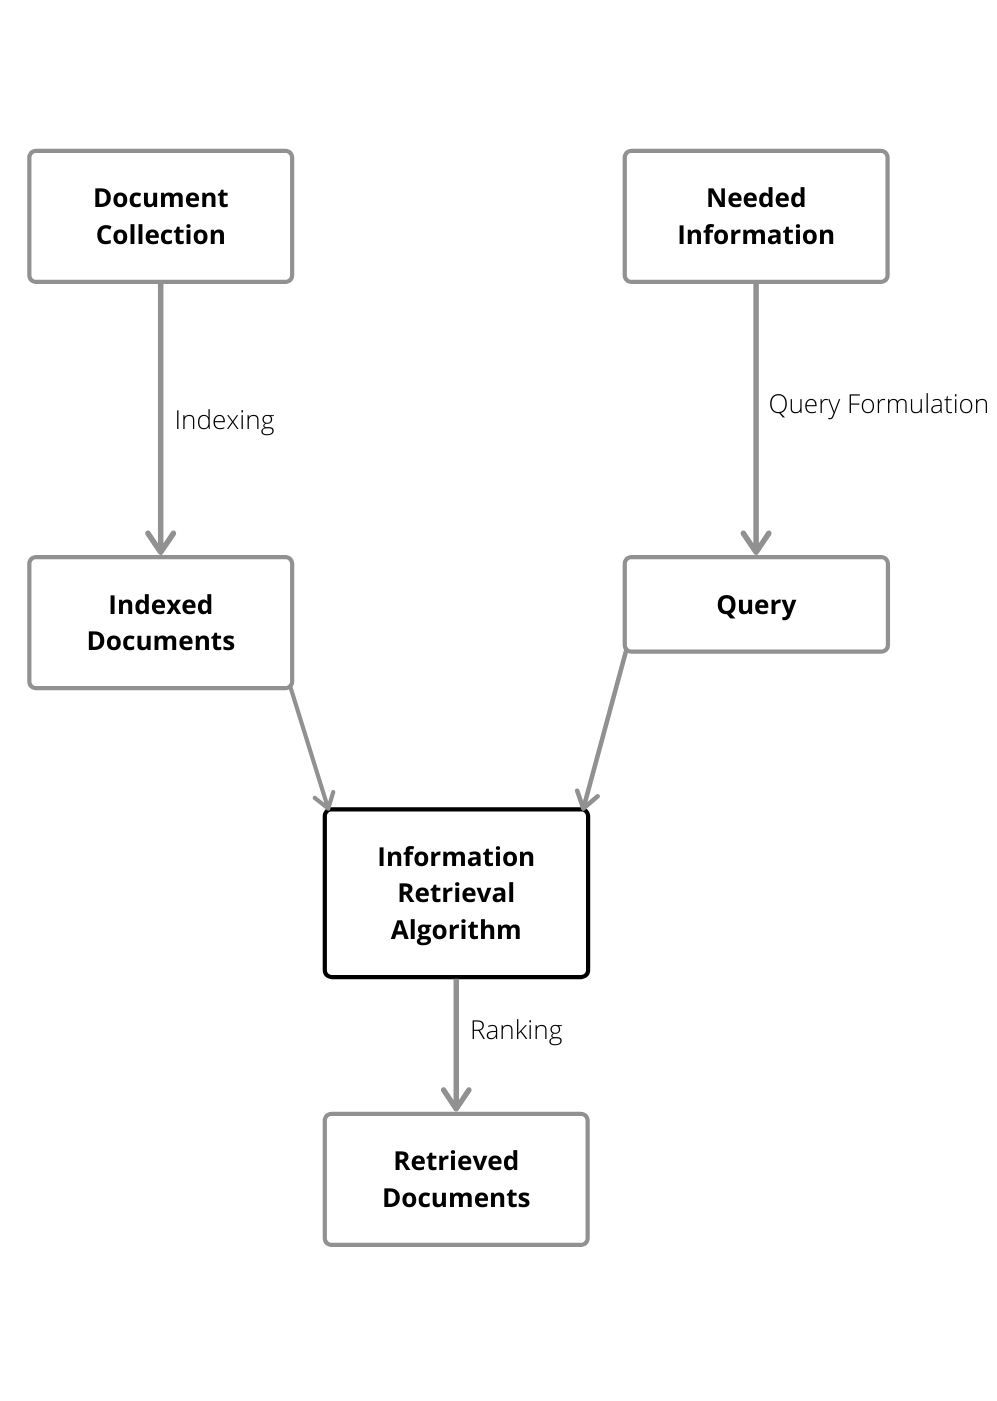
\includegraphics[width=0.6\linewidth]{Query.png}
        \centering
        \caption{Document Retrieval Scheme}
        \label{fig:dr-scheme}
    \end{figure}
    
    In the Text Retrieval Conference (TREC) competition~\parencite{trec2020overview}, they distinguish retrieval models into three categories:
    \begin{enumerate}
        \item \textbf{Traditional} - if it uses only TF-IDF/BM25 like models;
        \item \textbf{Neural} - if it employs some form of neural network based approach, but does not fall into \enquote{Neural using Language Models} category;
        \item \textbf{Neural using Language Models} - if it uses large scale pre-trained neural language models (LM).
    \end{enumerate}
    \noindent In this work, we have adopted this division. Nevertheless, we continue to deal only with the traditional models and neural models using LM, where the latter is the primary object of our interest.

\section{Traditional Approach}
\label{section:traditional-approach}
    Traditional approaches proceed from an empirically found law called \emph{Zipf's law}, which is commonly used as a model of the distribution of terms in a collection. This law
    states that the frequency  \emph{f\textsubscript{i}} of the \emph{ith} most common term in a collection is proportional to the inverse of its rank:
    
    \begin{equation}
        f_{i} \approx \frac{1}{i}
    \end{equation}
    
    \begin{figure}[H]
        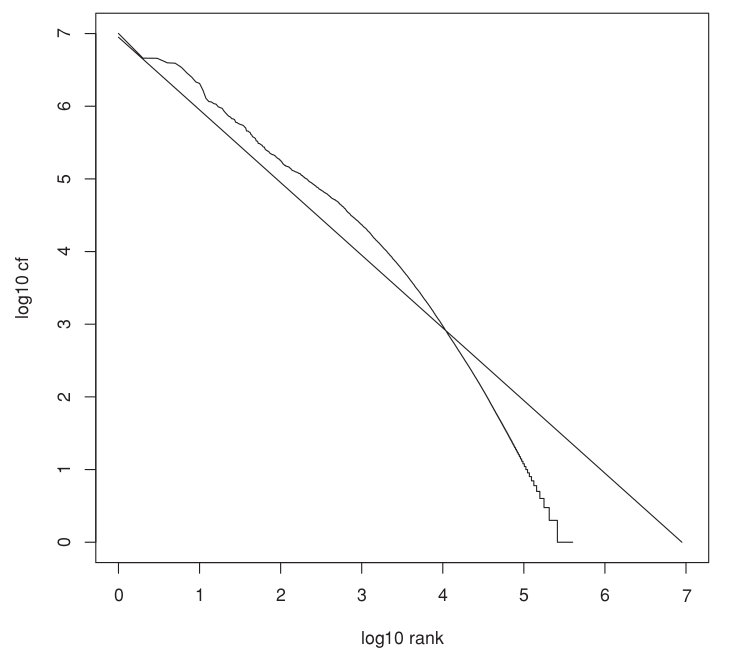
\includegraphics[width=0.6\linewidth]{zipf.png}
        \centering
        \caption[Zipf’s law]{Zipf’s law for Reuters-RCV1. Frequency is plotted as a function of frequency rank for the terms in the collection.~\parencite{manning2008introduction}}
        \label{fig:zipf}
    \end{figure}
    % law plati na AJ i na jinych jazycich?

\subsection{Term Frequency-Inverse Document Frequency (TF-IDF)}
\label{section:tf-idf}
    TF-IDF is a model (or weighting scheme more precisely) created with a knowledge of the Zipf's law. In the field of information retrieval, it can be considered as \enquote{evergreen} --- very popular and efficient method, which is implemented in a vast number of systems and applications as a search mechanism. TF-IDF is based on an underlying assumption that if terms from a given query are present more often in a document \emph{A} than in a document \emph{B}, then there is a closer relation between the query and document \emph{A} compared to the document \emph{B} (document \emph{A} should have a higher score). That is represented by the \emph{term frequency (tf)} part where a weight is assigned to each term \emph{t} in a document \emph{d} according to its frequency in the document.
    
    However, the words do not provide the same amount of information. Consider a document containing frequently the word \enquote{bird} and compare it with analogous knowledge only with a word \enquote{the}. Common words that are distributed over numerous documents provide only poor indication of a document's content. This introduces the second assumption represented by the \emph{inverse document frequency (idf)} part which scales the weight given by the \emph{term-frequency}. 
    \begin{equation}
        \emph{idf}_t = \log \frac{N}{\emph{df}_t}
    \end{equation}

    where:
    \begin{where}
        \item [N] is the total number of documents in a collection
        \item [df_{t}] is a document frequency of a term \emph{t} defined as the number of documents in the collection containing the term \emph{t}
    \end{where}
    
    Both parts can be combined into a single formula expressing the weight of the term \emph{t} in a document \emph{d}.
    \begin{equation}
        \label{equ:tfidf}
        \emph{tf-idf}_{t,d} = \emph{tf}_{t,d} \cdot \emph{idf}_{t}
    \end{equation} Mechanics of weighting can be summarized into 4 illustrative cases
    \begin{enumerate}
        \item term \emph{t} is assigned \textbf{highest} weight in document \emph{d} if \emph{t} occurs many times within a small number of documents;
        \item term \emph{t} is assigned \textbf{lower} weight in document \emph{d} if \emph{t} occurs fewer times, or occurs in many documents;
        \item term \emph{t} is assigned \textbf{lowest} weight in document \emph{d} if \emph{t} occurs in all documents;
        \item term \emph{t} is assigned weight \textbf{zero} in document \emph{d} if \emph{t} does not occur in the document at all.
       ~\parencite{manning2008introduction}
    \end{enumerate}

    By computing these weights for all terms per document from a collection, we can get the indexed collection (see Figure~\ref{fig:dr-scheme}). Each document \emph{d} will be represented by a vector of \emph{tf-idf}$_{d}$ weights, where each part of the vector corresponds to \emph{tf-idf} weight of term \emph{t} from a dictionary\footnote{the length of the vector is equal to the number of terms in the dictionary}. The document vector representation will be usually a very long (a lot of different words in the dictionary) and sparse (typically only a minority of existing words is used in a text of a given topic; also depends on the length of the text) vector.

    During the retrieval time when it is necessary to search for relevant documents given a query \emph{q}, the query is converted into \emph{bag of words (BOW)} vector representation (see Figure~\ref{fig:bow}). And since such a representation will have the same dimension as the representations of documents in the collection, score for query-document pair expressing the degree of relevance between them can be obtained by a simple dot-product. It is obvious that longer questions will reach a higher score due to the higher number of words, therefore both the document and query vectors are length-normalized (see equation~\ref{equ:q-d-score}).
    \begin{equation}
        \label{equ:q-d-score}
        sim(q, d) = \frac{V_{q} \cdot V_{d}}{|V_{q}| \cdot |V_{d}|}
    \end{equation}
    
    where:
    \begin{where}
        \item [|| \cdot ||] stands for the Euclidean norm~\parencite{manning2008introduction}
    \end{where}

    The BOW representation is one of the sparse representations because it usually has the vast majority of values equal to zero. In this case, both the query and the document are represented using BOW, which has some implications. The key simplification of this approach is that it does not include word order information or semantics information. To illustrate that, TF-IDF document representation of the document \enquote{Achilles is quicker than tortoise} is equal to the document representation of \enquote{Tortoise is quicker than Achilles} (see Figure~\ref{fig:bow}). Even though the documents have an opposite meaning, they are considered identical by having the identical document representation.~\parencite{manning2008introduction} This can be partially suppressed by using n-gram instead of individual words, which adds some semantic information.
    \begin{figure}[H]
        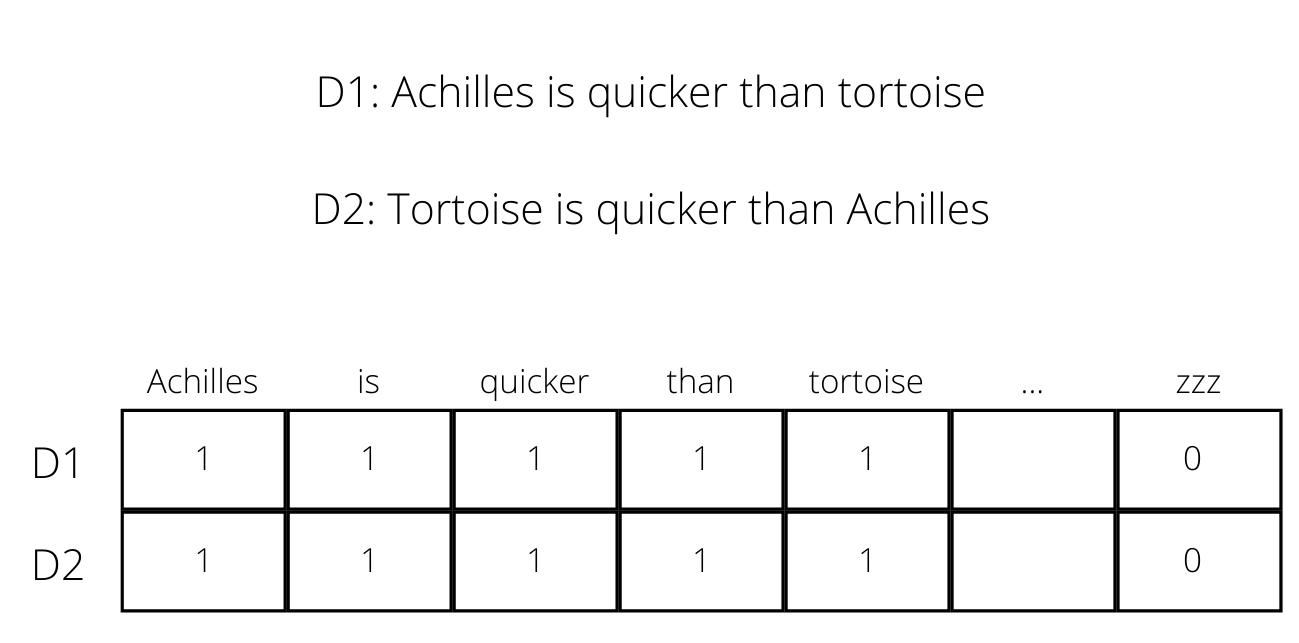
\includegraphics[width=0.6\linewidth]{Bag of Words.png}
        \centering
        \caption[Bag of words representation]{Bag of words representation. Dictionary is formed by words Achilles, is, \dots, zzz.}
        \label{fig:bow}
    \end{figure}


\subsection{Best Match 25 (BM25)}
\label{section:bm25}
    There is a more complex term weighting scheme called BM25~\parencite{robertson2009probabilistic} or Okapi weighting, which is expected to provide better results in practise. This approach proceeds from probabilistic information retrieval theory, but at the same time there is a strong resemblance to TF-IDF. The relevance of the document \emph{d} to the query \emph{q} is expressed as
    \begin{gather} \label{equ:bm25}
        \emph{BM25}_{q, d} = 
        \log \emph{idf}_t
        \cdot \frac{(k_1 + 1) \emph{tf}_{t, d}}{k_1((1-b) + b \cdot (L_d / L_{avg})) + \emph{tf}_{t, d}} 
        \cdot \frac{(k_3 + 1)\emph{tf}_{t, q}}{k_3 + \emph{tf}_{t, q}}.
    \end{gather}

    The BM25 can be broken up into 3 terms. The first term is the inverse document frequency which approximates the missing user-generated relevancy judgments. In case relevancy judgements are available, the following full form (equation~\ref{equ:bm25-rel}) can be used
    \begin{equation}
        \label{equ:bm25-rel}
        \log \frac{(|\emph{VR}_t| + 0.5) / (|\emph{VNR}_t| + 0.5)}{(\emph{df}_t - |\emph{VR}_t| + 0.5) / (N - \emph{df}_t - |\emph{VR}| + |\emph{VR}_t| + 0.5)}
    \end{equation} 
    
    where:
    \begin{where}
        \item [|\emph{VR\textsubscript{t}}|] stands for the set of relevant documents to term \emph{t}
        \item [|\emph{VNR\textsubscript{t}}|] is the set of non-relevant documents to term \emph{t} according to user feedback~\parencite{manning2008introduction}
    \end{where}
    % the $|\emph{VR\textsubscript{t}}|$ stands for set of relevant documents to term \emph{t} and $|\emph{VNR\textsubscript{t}}|$ is the set of non-relevant documents to term \emph{t} according to user feedback.~\parencite{manning2008introduction}

    The second term represents the document term frequency and document length scaling. Document term frequency builds on the assumption of the term frequency from TF-IDF. BM25 compared to TF-IDF does not assume that a document \emph{A} containing 2,000 times relevant term \emph{t} is $2\times$ more relevant than a document \emph{B}, which contains only 1,000 times the same term \emph{t}. But the effect decreases rapidly after reaching a certain level of saturation. This level of saturation can be regulated by the positive tuning parameter \emph{k\textsubscript{1}}.
    \begin{figure}[H]
        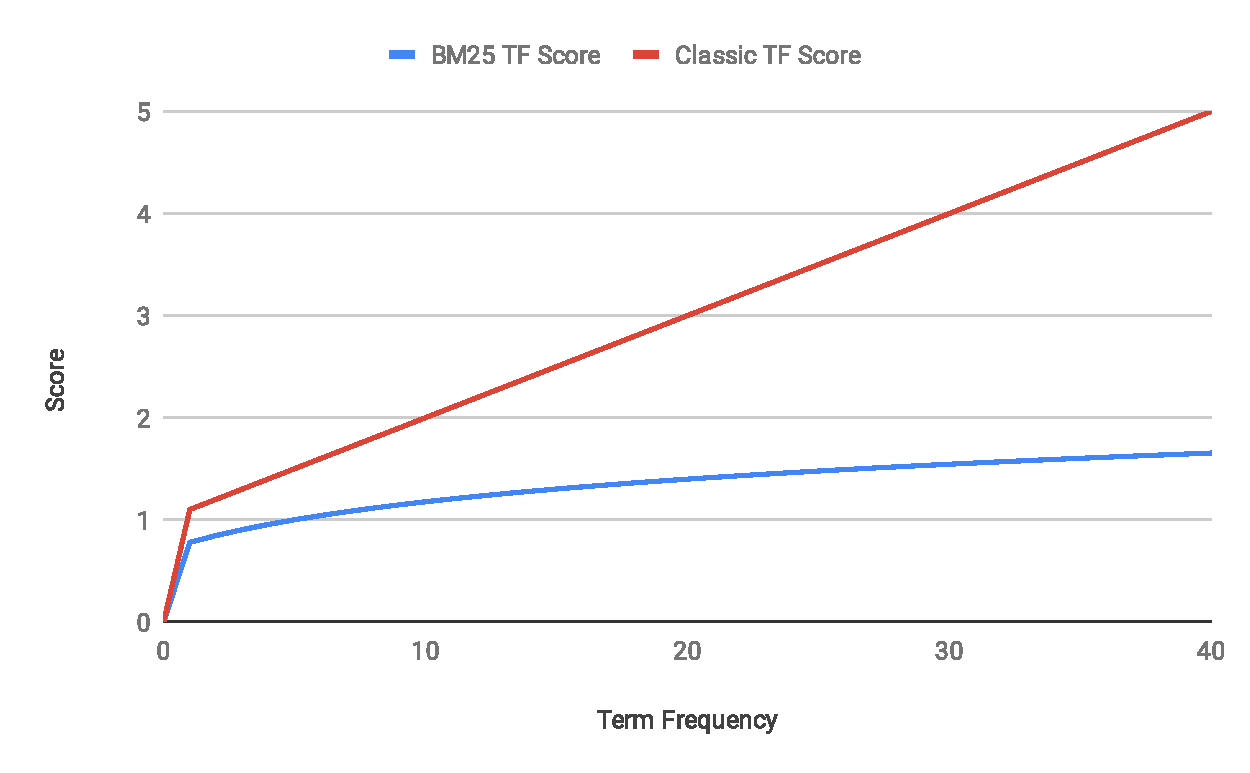
\includegraphics[width=0.8\linewidth]{tf-idf-vs-bm25.pdf}
        \centering
        \caption[Term frequency of TF-IDF vs. term frequency of BM25]{Term frequency of TF-IDF vs. term frequency of BM25. Adopted from~\parencite{tfidf-vs-bm25}}
        \label{fig:tf-idf-vs-bm25}
    \end{figure}

    \noindent In the TF-IDF weighting scheme document length is not directly involved, but in the case of BM25 it does not apply. The assumption is that if a term is observed in a short document then it has a bigger impact on the result than it would have in a longer document. Intuitively, assuming a single-word query \enquote{corruption} there is a higher chance that a short article is more relevant than an entire book if both documents contain the same number of that word. Size of the effect is calculated as a proportion of document length to an average length of all documents in the collection. The effect on the whole part is calibrated by a tuning parameter \emph{b} ranging from 0 (ignoring document length) to 1 (full influence of the document length).
    \begin{figure}[H]
        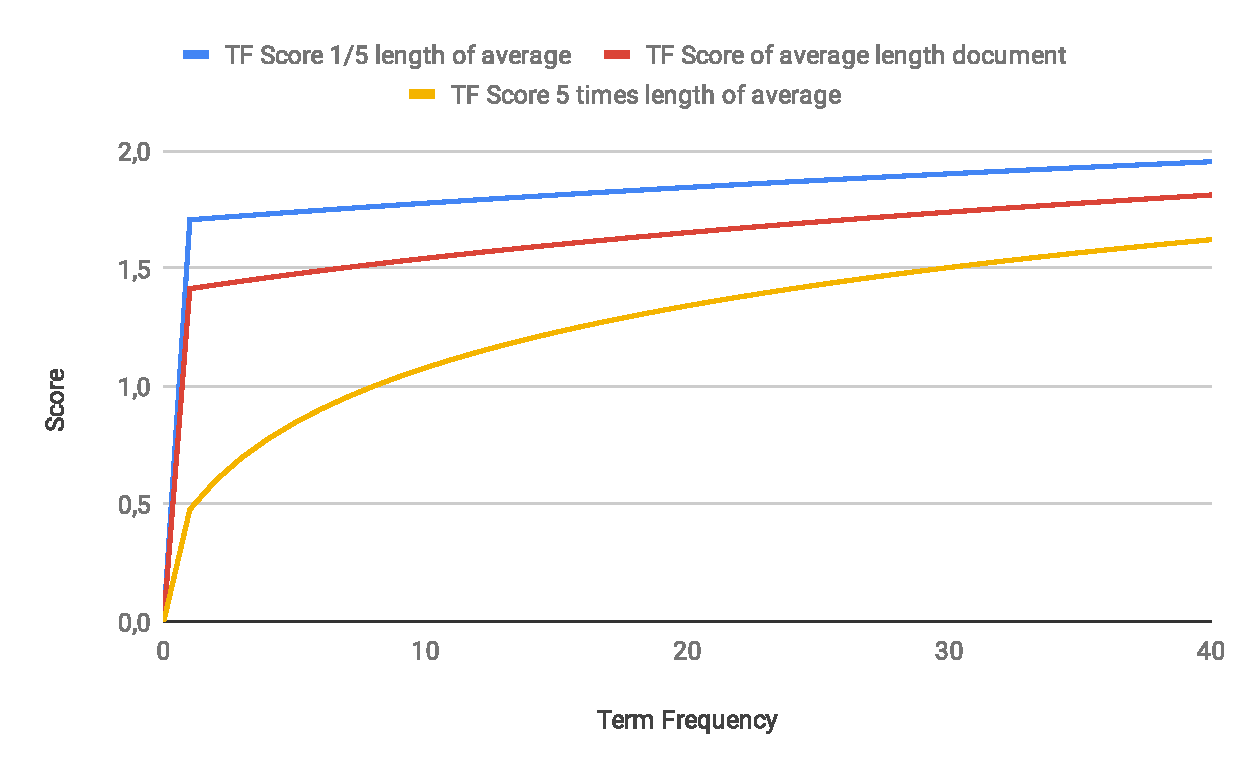
\includegraphics[width=0.8\linewidth]{bm25-doc-len.pdf}
        \centering
        \caption[Document length in BM25]{Document length in BM25. Adopted from~\parencite{tfidf-vs-bm25}}
        \label{fig:doc-len-bm25}
    \end{figure}
    % an influence of a single word 'corruption' is higher in an article than in a book.

    The third term scales the term frequency in the query. It has the analogical
    form as the document term frequency. Since queries are usually much shorter than documents, a simplified formula can be used. However, if the query is longer, such as a full paragraph, it may be more appropriate to use the full formula as in the second part of the equation~\ref{equ:bm25}.~\parencite{manning2008introduction}
    
    Further in the thesis I will refer to the models described in this section as TF-IDF-like models, as they are in principle very similar.
    % the returns of \emph{BM25} diminish with the growing \emph{term frequency} very rapidly after


\section{Language Modelling}
\label{section:language-modelling}
    A language model (LM) is a general name for statistical models which are able to predict the probability of a next word given some text input, simply put. More formally, it can be described as a probability distribution over sequences of tokens. Then the probability of a sequence \emph{t} can be expressed as a product of conditional probabilities 
    \begin{equation}
        \label{equ:LM-ngram}
        p(t) = \prod_{i=1}^{n}p(t_{i}|{t_1,\dots, t_{i-1}})
    \end{equation}
    
    \noindent Depending on the definition of the token, LM can be of different types. In case the token is a word, then the LM is called an unigram model and the probability of each word depends only on its own probability in the document or corpus
    \begin{equation}
        p(t) = \prod_{i=1}^{n}p(t_{i})  
    \end{equation}
    Generally, tokens can be modelled as \emph{n-grams} (see equation~\ref{equ:LM-ngram}), then the mechanics of using them in the model can differ, which leads to other types of LM's. %https://searchenterpriseai.techtarget.com/definition/language-modeling
    
    In information retrieval context, the LM's are used for some time already. The use is based on the idea that a document is relevant to a query if the LM of the particular document is likely to generate the query, which happens in the case if the document contains the query words often.~\parencite{manning2008introduction} One can notice a clear relation to traditional TF-IDF approaches in the idea.
    
    \begin{figure}[H]
        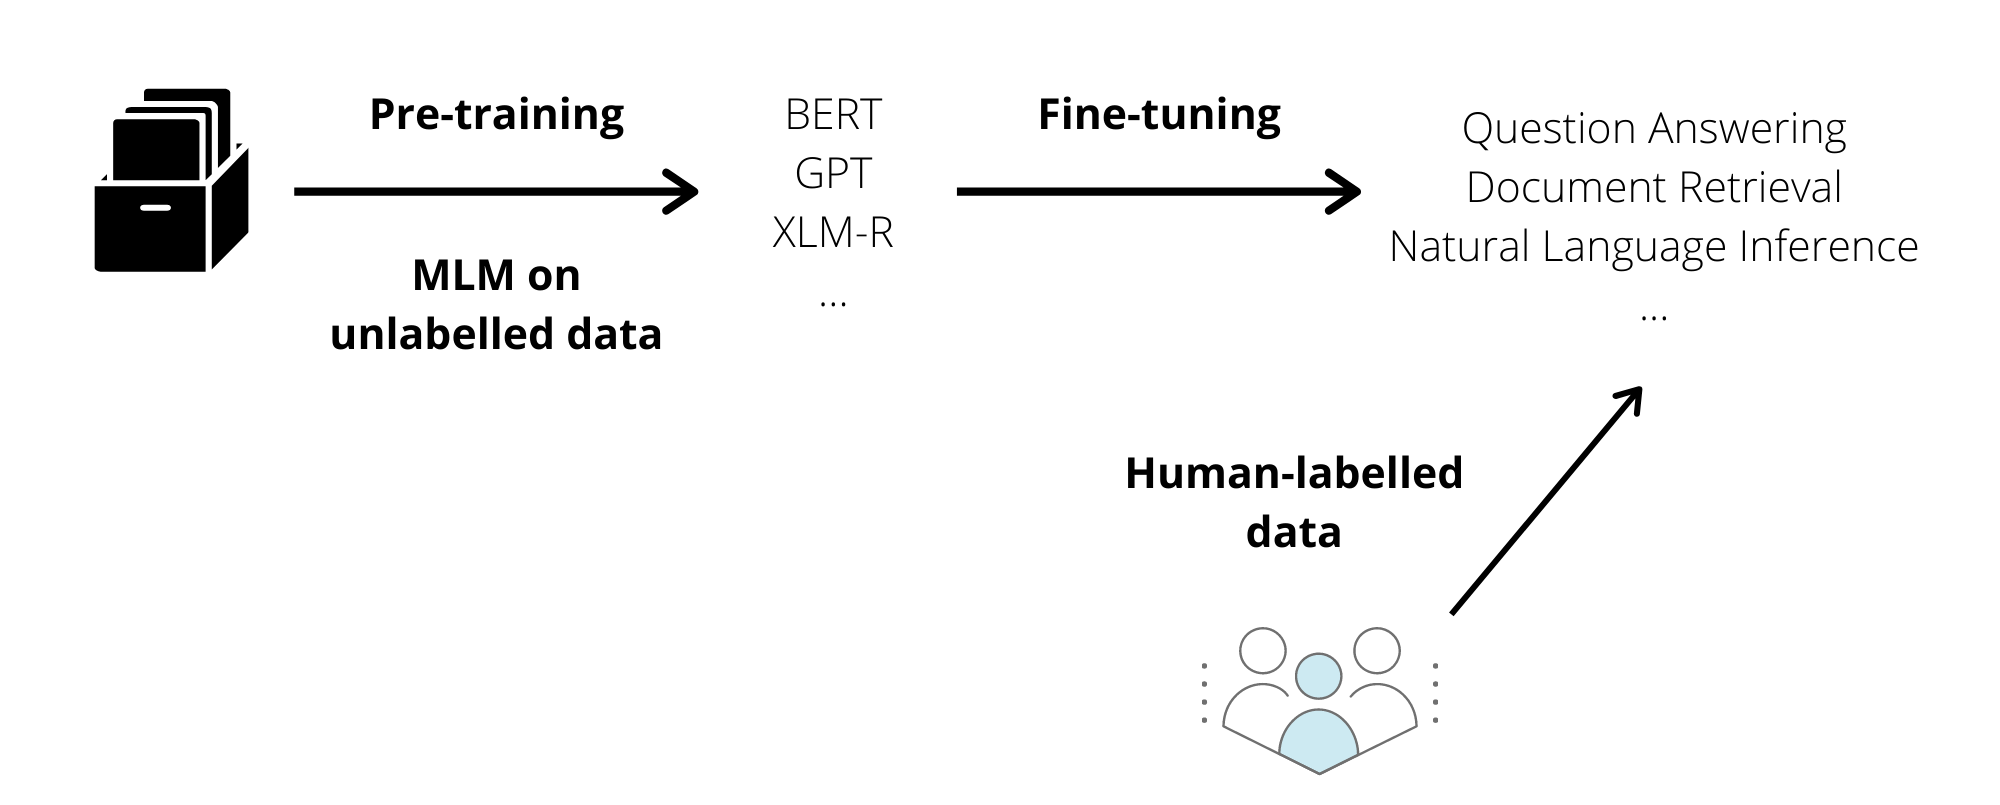
\includegraphics[width=0.85\linewidth]{transfer-learning.png}
        \centering
        \caption[Transfer learning]{Transfer learning. Adapted from~\parencite{ruder2021lmfine-tuning}}
        \label{fig:transfer-learning}
    \end{figure}
    
    Even though the LM's can be used \enquote{directly} for document retrieval (see query likelihood model in~\parencite{manning2008introduction} for example), their use went in another direction recently. In that direction, which is characteristic of the whole NLP field, LM's are primarily used for generating a rich contextual representation of texts that are consequently used as input features for other task-specific models, which are further trained (finetuned).~\parencite{ruder2021lmfine-tuning} This transfer learning based approach both enables to utilize huge and expensive to train LM's and significantly improve the state-of-the-art on various downstream tasks. This paradigm has also been established in the field of information retrieval, and recent work suggests that even here this approach can outperform traditional baselines.~\parencite{trec2020overview,Lee_2019_ict,Karpukhin_2020}.
    In the vast majority of cases, LM's are currently implemented using Transformer architecture and trained on a huge amount of data (see section~\ref{section:transformers}).


\subsection{One Model to Rule Them All!}
\label{section:transformers}
    Since 2017, the NLP world is dominated by a family of models called Transformers. They were firstly introduced in~\parencite{vaswani2017attention} and later become widely popular with their variations as BERT~\parencite{devlin2018bert} or GPT-2~\parencite{radford2019language}. There exist an overwhelming number of more or less different variants, which implementations can be found in Hugging Face's library called Transformers.~\parencite{wolf-etal-2020-transformers} 
    
    Transformer models got very rapidly adopted and applied to a diverse spectrum of tasks. From machine translation, question answering and document retrieval to non-NLP tasks as well. Transformers enable to model sequences --- often called sequence-to-sequence models --- and due to better parallelization offers faster processing compared to previously very frequently used recurrent neural networks (RNN).
    
    The transformer architecture is composed of an encoder and a decoder unit (see Figure~\ref{fig:transformer-arch}). Both units contain 6 repeatedly stacked identical layers. Each layer consists of a self-attention layer followed by a normalization layer and a fully connected feed-forward layer with a normalization layer. For both sub-layers there is a residual connection present.
    \begin{figure}[H]
        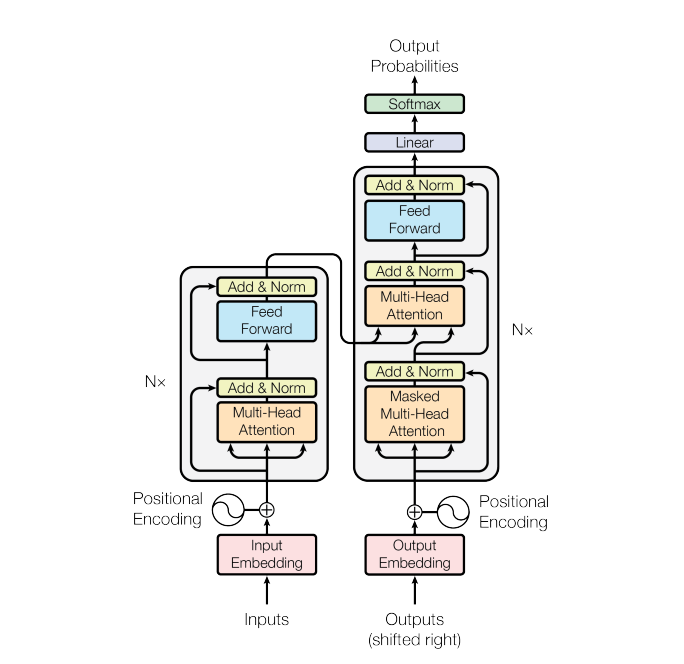
\includegraphics[width=0.8\linewidth]{Transformer-architecture.png}
        \centering
        \caption[Transformer architecture]{Transformer architecture. Encoder on the left and decoder on the right.~\parencite{vaswani2017attention}}
        \label{fig:transformer-arch}
    \end{figure}
    
    In addition to the encoder, the decoder contains a third sub-layer, which performs multi-head attention over the output from the encoder stack. Self-attention layers of the decoder are modified, so they have access to only already decoded positions (prediction for position \emph{i} can depend only on the known outputs at positions less than \emph{i}). This masking is crucial as it keeps the model auto-regressive (with leftward information flow) in all steps. Therefore, every prediction at a position \emph{i} depends only on the known outputs from positions before \emph{i}.
    
    % Decoder structure is very similar only with one additional self-attention layer followed by a normalization layer block in each of the decoder layer, which performs multi-head attention over the output from the encoder stack. Self-attention layers in the decoder are modified that it enables to attend to only already decoded positions. This masking is crucial as it keeps the model auto-regressive (with leftward information flow) in all steps. Therefore, every prediction at a position \emph{i} depends only on the known outputs from positions before \emph{i}.


\subsubsection{Attention Mechanism}
\label{section:attention-mechanism}
    The very core of the transformer is an attention mechanism. 
    \textbf{Self-attention} of a word in an input sentence provides its relation to all the other words in the input sentence as it is depicted in Figure~\ref{fig:attention-sentence}.
    \begin{figure}[H]
        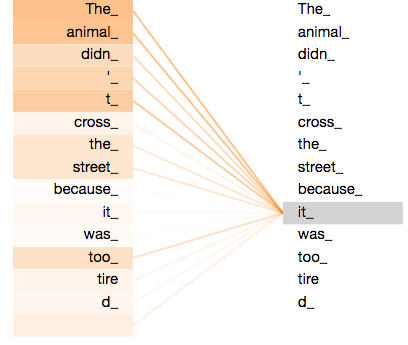
\includegraphics[width=0.6\linewidth]{attention-1layer.png}
        \centering
        \caption[Illustrated attention mechanism]{Illustrated attention mechanism.~\parencite{alammar_transformer}}
        \label{fig:attention-sentence}
    \end{figure}
    
    Self-attention works with 3 matrices: query \emph{Q}, key \emph{K} and value \emph{V} which represent certain abstractions. These matrices are obtained by projecting each word, respectively its word embedding, using trained weight matrices for each particular abstraction. The self-attention of a word is computed by multiplying its corresponding query vector from \emph{Q} and the key vector from \emph{K}. This is normalized by dividing it by the square root of the dimension of the key vector and passing it through the softmax. Multiplying this softmax score with each value vector from \emph{V} and summing them results in the \textbf{scaled dot-product attention}.
    
    Instead of performing this scaled dot-product attention once, the \textbf{multi-head attention} mechanism calculates the scaled dot-product attention multiple times in parallel. This is done by creating a multiple of different \emph{Q}, \emph{K} and \emph{V} matrices with different learned linear projections. That will produce multiple different output attentions, which are concatenated and projected to the final output dimension.
    % Then  the scaled dot-product attention is computed using those matrices.
    \begin{figure}[H]
        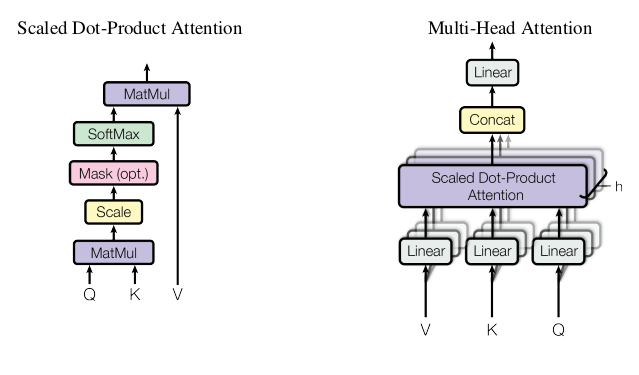
\includegraphics[width=0.8\linewidth]{attention.png}
        \centering
        \caption[Scaled Dot-Product Attention and Multi-Head Attention]{Scaled Dot-Product Attention and Multi-Head Attention~\parencite{vaswani2017attention}}
        \label{fig:attention}
    \end{figure}


\subsubsection{Positional Encoding}
\label{section:pos-encoding}
    % http://nlp.seas.harvard.edu/2018/04/03/attention.html#positional-encoding
    % https://kazemnejad.com/blog/transformer_architecture_positional_encoding/
    Since the transformer model does not process words in a sentence sequentially, but in parallel (all at once), it loses information about order. This is solved by the \textbf{positional encoding}, which provides a sense of position or order for each word. The positional encoding is a \emph{d}-dimensional vector with the same dimension as has word embedding and components computed by the following rule
    \begin{align} \label{equ:pos-encoding}
    \begin{split}
        PE_{pos, 2i} &= \sin(\frac{pos}{10\,000^{\frac{2i}{d}}}) \\
        PE_{pos, 2i+1} &= \cos(\frac{pos}{10\,000^{\frac{2i}{d}}})
    \end{split}
    \end{align}
    
    where:
    \begin{where}
        \item [\emph{pos}] is the desired position in the input sentence
        \item [\emph{d}] is the encoding dimension, which must be divisible by 2
        \item [\emph{i}] is the dimension. Each dimension of the PE vector corresponds to a sinusoid and the wavelengths form a geometric progression from $2\pi$ to $10\,000 \cdot 2\pi$ 
    \end{where}
    
    \noindent The positional encoding vector is then summed with a word embedding which explains the choice of dimension of PE vector.~\parencite{vaswani2017attention}
    
    \[
    PE_{pos} =
    \begin{bmatrix}
       \sin(\omega_{1}) \\ \cos(\omega_{1})  \\  \vdots \\ \sin(\omega_{d/2}) \\ \cos(\omega_{d/2})
    \end{bmatrix}
    \] 
    
    where $\omega_{j} = \frac{1}{10\,000^{2j / d}}$.

\subsection{BERTology}
\label{section:bertology}
    Bidirectional Encoder Representations from Transformers (BERT) presented in~\parencite{devlin2018bert} was designed to pretrain deep bidirectional representations from unlabeled data. These representations are obtained by implementing bidirectional self-attention that computes both with left and right context in all layers. This fundamental difference from unidirectional (left to right) models makes better use of pre-trained representations especially in approaches involving fine-tuning, they argue in the paper.
    
    \begin{figure}[H]
        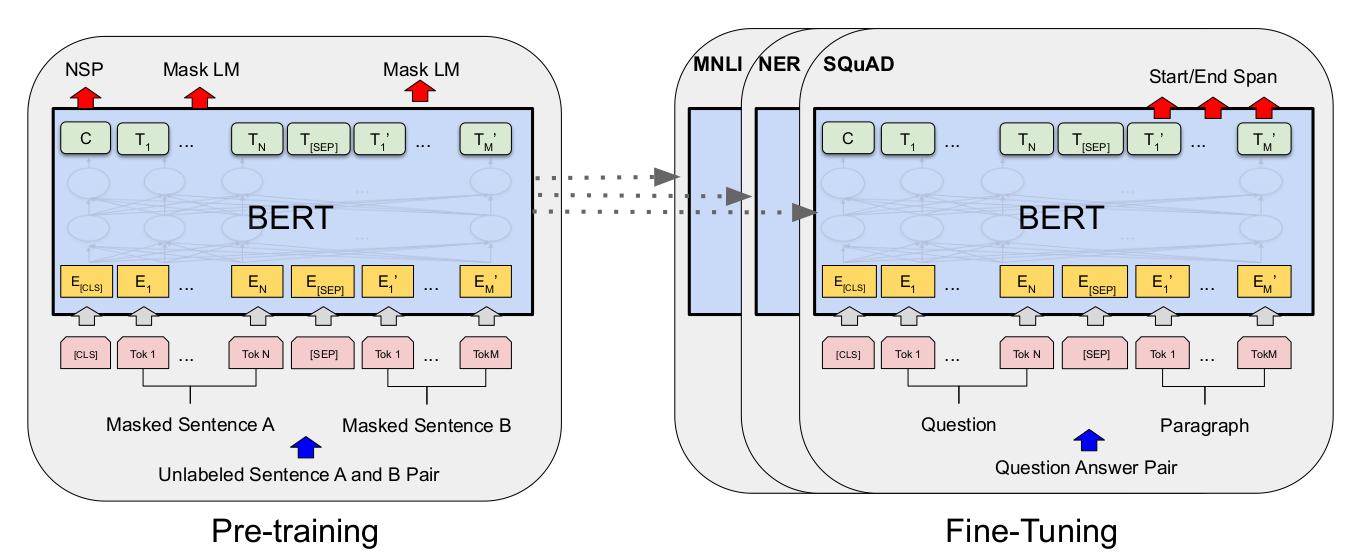
\includegraphics[width=0.95\linewidth]{bert.png}
        \centering
        \caption[Pre-training and fine-tuning procedures for BERT]{Overall pre-training and fine-tuning procedures for BERT. Apart from output layers, the same architectures are used in both pre-training and fine-tuning. The same pre-trained model parameters are used to initialize models for different down-stream tasks. During fine-tuning, all parameters are fine-tuned. [CLS] is a special symbol added in front of every input example, and [SEP] is a special separator token (e.g. separating questions/answers).~\parencite{devlin2018bert}}
        \label{fig:bert}
    \end{figure}
    
    BERT workflow consists of two steps: pre-trained on unlabeled data over different pre-training tasks and fine-tuning on downstream task (e.g. question answering or name entity recognition) using labeled data. So at the end, there was a fine-tuned model variation for each of the downstream task. The pre-training step is performed indirectly by using two pre-training tasks. The first is \textbf{masked language model (MLM)}, which randomly masks some of the tokens from the input and model tries to predict the original words in masked places based only on its context. The second is \textbf{next sentence prediction (NSP)}, where the task is to classify whether a two given sentences are neighbors or not.~\parencite{devlin2018bert} 
    
    The model architecture is a multi-layer bidirectional Transformer encoder based on the original Transformer implementation~\parencite{vaswani2017attention}. A benefit of this model is its unified architecture that differs minimally between pre-training and fine-tuning setup. 
    
    This model is so popular and widely used that it has led to the creation of a meta-study aptly named Bertology, which provides an overview of the accumulated knowledge about BERT.~\parencite{Rogers_2020}


\subsection{As many languages you know, as many times you are a language model}
\label{section:multiling-models}
    % Multilingual Language Model
    When working with text data, using various NLP techniques and especially expensive to train language models, one can notice a big disproportion. Only a very small number of languages have available data and thus pre-trained language models. Even in the small cluster of languages having the richest language resources, there is a clear gap between English and the rest of them (see Figure~\ref{fig:lang-dist}). Despite the data scarcity problem does not have an easy solution yet, there are some interesting research results that can help to reduce the impact of the gap. Training multilingual and cross-lingual models provide some of them.
    %have much favoured English language is compared to other languages.   
    \begin{figure}[H]
        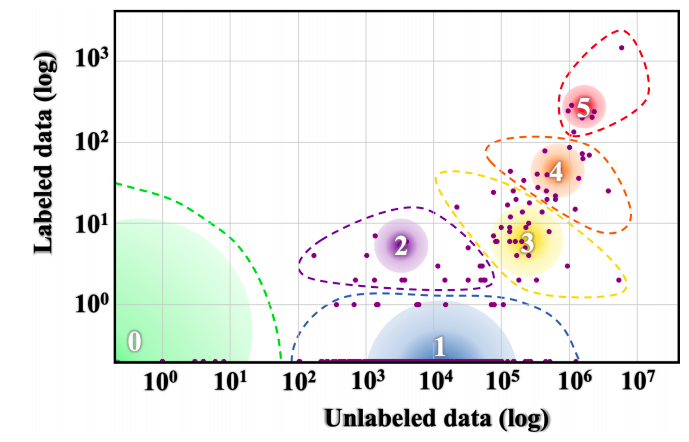
\includegraphics[width=0.8\linewidth]{language-dist.png}
        \centering
        \caption[Language Resource Distribution]{Language Resource Distribution: The size of the gradient circle represents the number of languages in the class. The color spectrum VIBGYOR, represents the total speaker population size from low to high. Bounding curves used to demonstrate covered points by that language class.~\parencite{Joshi_2020}}
        \label{fig:lang-dist}
    \end{figure}
    
    Pre-training of LM is performed indirectly by using pre-training tasks. In addition to the above \textbf{MLM} and \textbf{NSP}, there exists other pre-training tasks for example \textbf{causal language modelling (CLM)}, which models the probability of a word given previous words in a sentence. Usually, there is no need for labelled data in the pre-training tasks as they have an unsupervised nature. This becomes a great benefit given the fact that only a minority of existing text data is labelled and that LM needs a substantial amount of data for pre-training. 

    % A typical pre-training task is a \textbf{masked language model (MLM)}, which randomly masks some of the tokens from the input and model tries to predict the original word of the masked word based only on its context; \textbf{next sentence prediction (NSP)} where the task is to classify whether a two given sentences are neighbors or not.~\parencite{devlin2018bert} or \textbf{causal language modelling (CLM)}, which models the probability of a word given previous words in a sentence. Usually, there is no need for labelled data in the pre-training tasks as they have an unsupervised nature. This becomes a great benefit given the fact that only a minority of existing text data is labelled and that LM needs a substantial amount of data for pre-training. 
    
    The process of pre-training multilingual LM is very similar as for pre-training monolingual LM's. The primary and obvious difference is that multilingual ones are trained with data of multiple languages with the goal to learn a coexisting vector-space representations for them. It was shown that low-resource language often benefits from training together with a higher-resource language, especially when it shares a significant fraction of its vocabulary.~\parencite{lample2019crosslingual} In addition to universal pre-training tasks, there exist also tasks specific to multilingual setup. For example, in~\parencite{lample2019crosslingual} they presented \textbf{translation language modelling (TLM)} task, which utilizes parallel data resulting in strong cross-lingual features provided by the model.
    
    The choice of pre-training tasks can significantly affect the model, its vector space and thus the provided representations, especially in the multilingual setup. The term \emph{cross-linguality} refers to the property of the model to create general text representations across languages. Simply put, given two semantically very similar words in different languages, the model should provide representations which are also very close.
    
    Monolingual models are in most cases superior in performance compared to multilingual models.~\parencite{Martin_2020,Dumitrescu_2020} Nevertheless, XLM-RoBERTa (XLM-R) proposed in~\parencite{Conneau_2020} is a multilingual model trained on a very large scale regarding the data (2.5~TB) as well as the number of languages (one hundred). It also showed that a multilingual model can be competitive with a monolingual ones on some tasks while providing solid cross-lingual features. The performance is quite surprising as the model was trained only on unsupervised data using MLM without an explicit training signal providing information about the language of a given text such as parallel data provides. Further findings shows that if you train a large enough network on a large enough amount of data, you can get equivalent performance to a monolingual model, while being able to develop model that can do well on multiple languages at once.~\parencite{li2021scaling}
    
    Considering Czech language, XLM-R's Czech reading comprehension was examined in~\parencite{Mackov_2020_czech_xlmr}, where the XLM-R showed competitive performance compared to monolingual models even without training on parallel data. And a very recently released monolingual Czech model Czert \parencite{sido2021czert}, which in most tasks surpasses the performance of multilingual models, but unfortunately the comparison with XLM-R is missing.

\subsection{Distillation}
\label{section:distillation}
    In recent years, there has been a trend towards increasing language models, which produced 8.3 billion parameters Megatron LM~\parencite{shoeybi2019megatronlm} and currently the biggest 175 billion parameters GPT-3~\parencite{brown2020language-gpt3}. They provide significant improvements in various NLP tasks --- the latter was not even made public in its full scale due to safety-related concerns --- but for a very high price.~\parencite{Schwartz_2020} 
    %https://openai.com/blog/openai-api/
    The substantial size of these models also makes them slower and less convenient due to a high computational and memory requirements. This can significantly reduce the possibility of their deployment, particularly in document retrieval, where the run time is expected to be near real-time.
    
    \begin{figure}[H]
        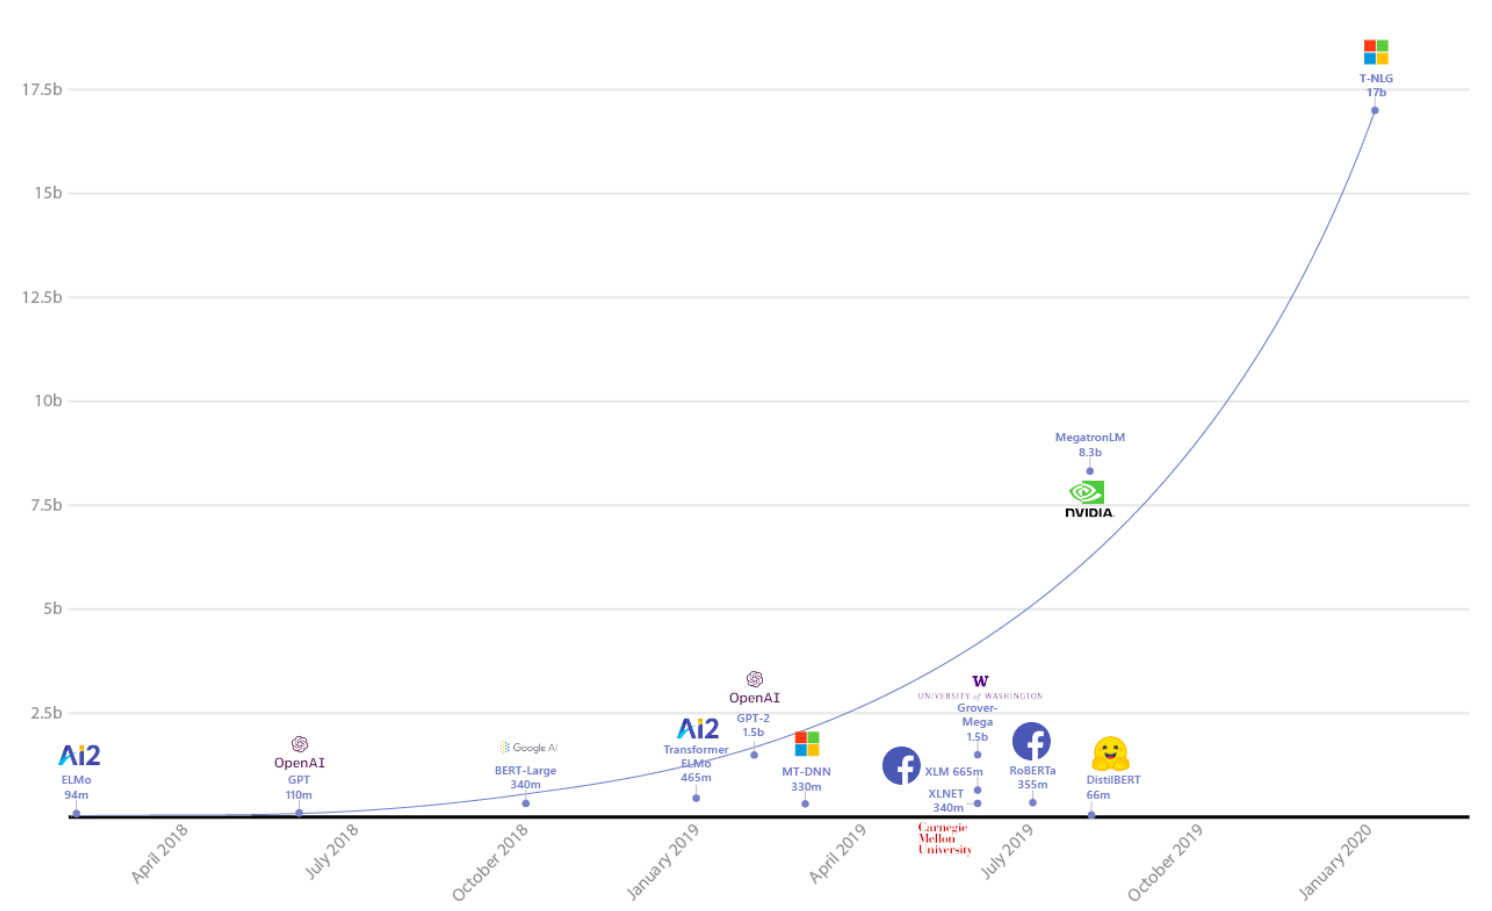
\includegraphics[width=1\linewidth]{lang-models-comparison.png}
        \centering
        \caption[Language models comparison by number of parameters]{Models compared by a number of parameters (currently the biggest model GPT-3 with a significant margin is not included).~\parencite{language-models-comparison}}
        \label{fig:model-parameters-comparison}
    \end{figure}
    
    Recent results showed that it is possible to reach a very similar performance on many downstream tasks using much smaller LM pre-trained with \emph{knowledge distillation technique}.~\parencite{Sanh2019DistilBERTAD} Knowledge distillation is a compression technique presented in~\parencite{distillation} and later applied to neural networks in~\parencite{hinton2015distilling}. This technique is based on an elegant idea where the smaller (distilled) model (student) is trained to reproduce the behavior of a larger model (teacher) or an ensemble of models. 
    
    In the case of BERT, the distilled version is created by lowering the number of layers, removing token-type embeddings and poolers, while the general architecture is preserved. An important step is the initialization, which affects the speed of convergence of the student model. Due to the common dimensionality, the student model is initialized by the teacher model weights, which provides fast convergence.~\parencite{Sanh2019DistilBERTAD}
    
    Another interesting applications of distillation are proposed in~\parencite{hofstaetter2020_crossarchitecture_kd}, where they use cross-architecture knowledge distillation to improve the effectiveness of the neural passage ranking models with efficient query latency; or in~\parencite{Reimers_2020-distillation-multiling}, in which distillation is used for transforming monolingual sentence embeddings into multilingual by aligning vector spaces between languages.

\subsection{Tokenization}
\label{section:tokenization}
    In NLP, tokenization is a process of splitting a text into smaller units called tokens. A token can be a word, subword, or character. The key motivation is to have a finite set of symbols (vocabulary) which parts can be combined to get the desired result. Simple to describe, yet in practice it is a more complicated problem. 
    
    There is a tradeoff between the size of the vocabulary affecting the computational complexity and performance of the model. Having tokens on the level of characters will result in  a small memory footprint as there is a relatively small number of existing characters, but it will be very tricky to learn a  general representation of a single character. That can result in lower performance of the model. On the other hand, having tokens on the level of words will increase the memory footprint and thus also the computational complexity (consider different endings for a single word stem), but it will be much easier to learn the representation of a whole word, which will have a positive effect on the performance of the model.
    
    Good tradeoff provides subword tokenizers, which keep a reasonable vocabulary size while learning a meaningful context-independent representation is enabled. One of such tokenizers is the algorithm called \textbf{WordPiece}, which is used for BERT transformer model. WordPiece initializes the vocabulary with every character present in the training text and it gradually learns a given number of merge rules (see Algorithm~\ref{alg:wordpiece-tokenizer}).
    
    \begin{algorithm}[]
        \textbf{Initialize}: Initialize the vocabulary with all the characters present in the training text. 
        \\
        \textbf{Step1}: Build a language model on the training data using the vocabulary from the previous step.
        \\
        \textbf{Step2}: Generate a new subword unit (wordpiece) by combining two units out of the current vocabulary to increment the vocabulary by one. Choose the new subword unit out of all the possible ones that increases the likelihood on the training data the most when added to the model.
        \\
        \textbf{Step3}: Go to Step2 until a predefined limit of subword units is reached or the likelihood increase falls below a certain threshold.
     \caption[WordPiece Algorithm]{WordPiece Algorithm~\parencite{wordpiece-tokenizer}}
     \label{alg:wordpiece-tokenizer}
    \end{algorithm}
    
    Similarly to WordPiece, \textbf{Byte Pair Encoding (BPE)} tokenizer also gradually learns a given number of merge rules, but in a different way.~\parencite{BPE-tokenizer} BPE tokenizer assumes the data are already splitted into words. Having words represented as a sequence of characters, the vocabulary is initialized in the same way as for the WordPiece algorithm. BPE then iteratively counts all subword pairs and replace each occurrence of the most frequent pair (e.g. \enquote{A}, \enquote{L}) with a new symbol \enquote{AL}. Frequent subwords or even whole words are eventually merged into a single token. The final vocabulary size is equal to the number of distinct characters in the training data (the size of initial vocabulary) plus the number of merge rules, which is the only hyperparameter of the algorithm. One can see the key difference is in choosing a merge rule step. BPE chooses simply the most frequent subword pair in the data, compared to the pair maximizing the likelihood chosen by WordPiece.
    
    Tokenizers stated above assume either the training text is already splitted into words or it can be relatively easily done by some pre-tokenizer that assumes words are separated by whitespace. This approach becomes a problematic at the moment we try to tokenize a language, which does not use whitespace to separate words. A possible solution is to use pre-tokenizer created for that particular language. More general solution is to use \textbf{SentecePiece} tokenizer which enables to train subword models directly from raw sentences by treating whitespace as one of the tokens inside the vocabulary. SentecePiece implements an optimized BPE~\parencite{BPE-tokenizer} with $\mathcal{O}(n\log n)$ due to using priority queue and unigram language model~\parencite{unigram-toknizer}. Besides that, SentecePiece provides further functionality --- e.g. manages a vocabulary to id mapping to directly convert the input text into an id sequence; it enables customizable character normalization; it makes the reproduction of preprocessing steps easy by embedding all the rules and parameters into self-contained model by design --- which makes it end-to-end system that does not depend on any language-specific processing. Due to that, SentecePiece is a very convenient tokenizer for multilingual models.
    
    Those tokenizers mentioned above are only a subset of the existing ones. A nice overview of subword tokenizers as well as their implementation provides HuggingFace library.~\parencite{wolf-etal-2020-transformers}


% ----------------------------------------------------------------------------------------------------------
% HYBRID APPROACH
% ----------------------------------------------------------------------------------------------------------
\section{Hybrid Approach}
\label{section:hybrid-approach}
    Another approach to document retrieval is the \emph{hybrid approach} that combines traditional methods and language models. With the advent of transformer models, there occurred many works experimenting with this approach, for example~\parencite{nogueira2019passage} or other works implementing integrated systems such as Bertserini~\parencite{bertserini} or Birch~\parencite{birch}.
    
    % Systems generally followed a multi-step process: They 1) identified the type of the answer based on the question (“who”, “when”, “where”, etc); 2) used IR to retrieve relevant documents based on question similarity; 3) performed a shallow parse of the documents; and 4) detected entities of the corresponding type in the context; if no entity was found, they fell back on heuristics. This general combination of IR + document processing still is at the heart of open-domain QA systems today (Chen et al., 2017).
    % https://www.aclweb.org/anthology/P17-1171/?utm_campaign=NLP%20News&utm_medium=email&utm_source=Revue%20newsletter
    
    The underlying idea behind this approach is to divide the task of DR into two parts as was presented in~\parencite{chen2017reading-drqa}. In the first part, usually called \emph{retriever}, is performed a rough pre-selection of documents using typically faster and more efficient traditional methods, which allow to realize retrieval in sublinear time using the inverted index. In the second part, computationally more demanding neural model is used to re-rank the relatively small number of already pre-selected documents. That part is usually called the \emph{reader} (see Figure~\ref{fig:hybrid-approach}). 
    \begin{figure}[H]
        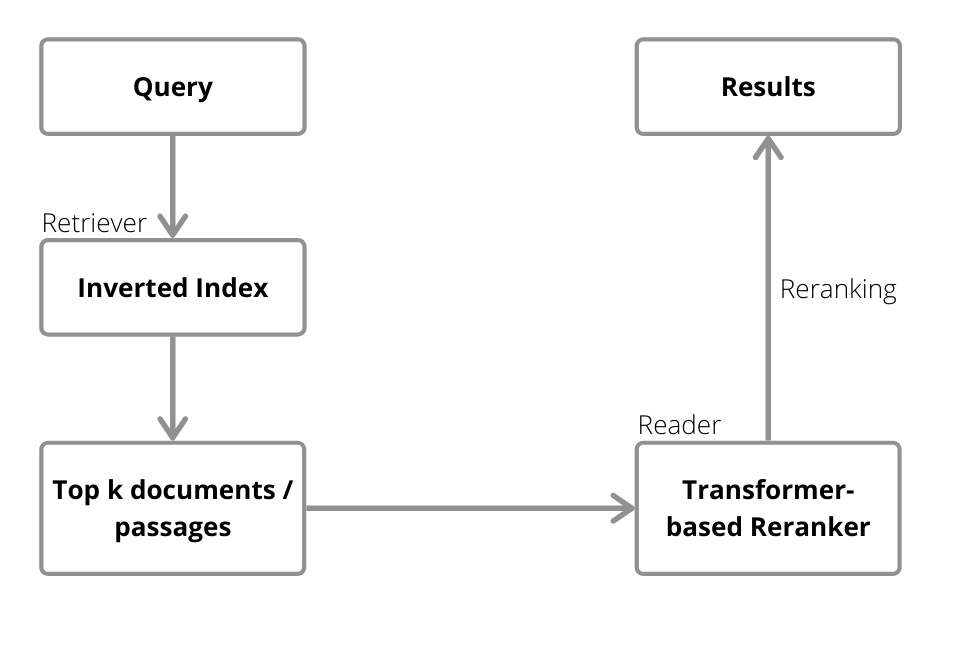
\includegraphics[width=0.6\linewidth]{Hybrid Approach.png}
        \centering
        \caption{Hybrid Approach Scheme}
        \label{fig:hybrid-approach}
    \end{figure}
    
    In general, specific document retrieval pipeline depends on the task and the data we are working with. Therefore, the pipeline can be of arbitrary complexity and it can have more steps than only retrieval and re-ranking. In~\parencite{diggelmann2020climatefever} their retrieval pipeline utilizes natural granularity of textual data and consists of three steps: 
    \begin{enumerate}
        \item document retrieval using BM25 operating on full-length Wikipedia articles, returning top \emph{d} documents;
        \item sentence retrieval using pre-trained LM for generating sentence embeddings and returning top \emph{s} sentences;
        \item sentence re-ranking using the same LM for computing relevance scores of claim-sentence pairs and providing re-ranked top \emph{s} sentences
    \end{enumerate}

    The BM25/TF-IDF retrievers are very efficient and proven by a wide range of applications in industry as they provide reasonable trade-off between latency and accuracy. Their popularity is also evident from the tables with the submitted solutions of the MS MARCO passage and document ranking tasks\footnote{\url{https://microsoft.github.io/msmarco/}}.
    
    However, they have a clear disadvantage as the quality of the retrieved results depends on the performance of the retriever, which lacks the semantic and contextual understanding, as was described in section~\ref{section:tf-idf}. Although there exists techniques, that try to mitigate the term mismatch error by enriching documents with potential query terms, presented in~\parencite{nogueira2019document, nogueira2019doc2query} or replace the BM25's term frequency with LM-estimated term importance~\parencite{dai2019contextaware}, their effects are limited.  End-to-end neural retrieval that provides deeply-contextualized semantic representations of queries and documents bridging the widespread problem of vocabulary mismatch can offer a better solution.


% ----------------------------------------------------------------------------------------------------------
% NEURAL APPROACH
% ----------------------------------------------------------------------------------------------------------
\section{Neural Approach}
\label{chapter:neural-approach}
    With the successful application of neural models in combination with traditional models, the research community focused on the end-to-end neural retrieval, also referred to in the literature as dense retrieval.
    Their efforts crystallized into several different paradigms (see Figure~\ref{fig:neural-approach-paradigms}).
    \begin{figure}[H]
        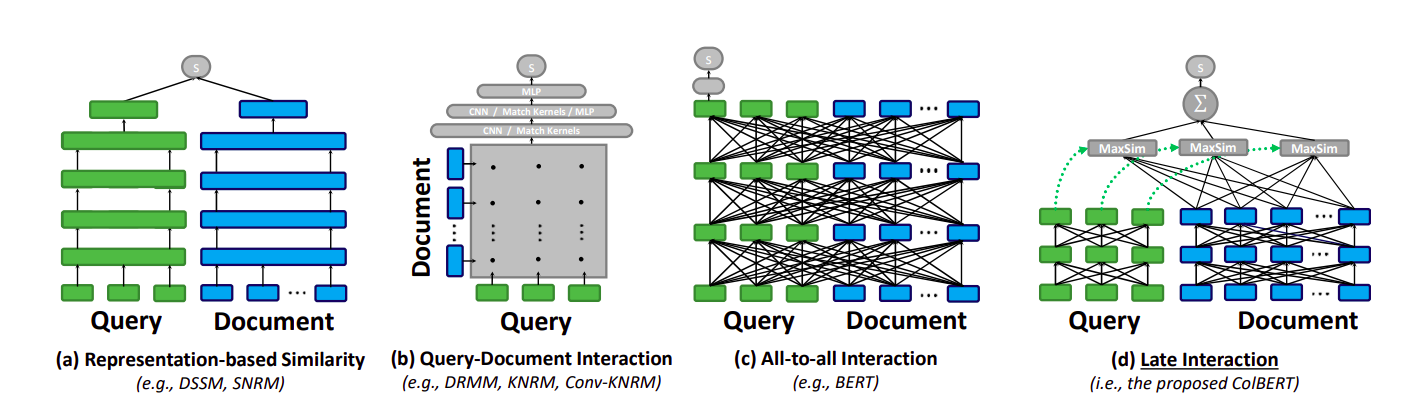
\includegraphics[width=1\linewidth]{neural-dr-types.png}
        \centering
        \caption[Query–document matching paradigms in neural IR]{Schematic diagrams illustrating query–document matching paradigms in neural IR.~\parencite{colbert_2020}}
        \label{fig:neural-approach-paradigms}
    \end{figure}


\subsection{Cross-Attention Paradigm}
\label{section:cross-attention}
    This paradigm enables to model interactions between words within as well as across a query and document at the same time, see Figure (c) in~\ref{fig:neural-approach-paradigms}. This is realized by concatenating the query with the document separated by some special token and inputting them into the transformer model. A linear layer or multilayer perceptron can be appended to the transformer predicting the relevancy score between the query and document or binary relevant/non-relevant output signalizing whether the document is relevant to the query.
    
    This interaction-based paradigm tends to be more effective compared to two-tower paradigm from section~\ref{section:two-tower} as it might be very hard to represent a single document by a single low-dimensional vector, especially when the document is long and contains a mixture of different topics.~\parencite{mitra-intro-to-ir}
    %https://arxiv.org/pdf/1911.11951.pdf stance detection
    
    On the other hand, it would be impossible for the model to work with reasonable latency, especially in the case of large collections of documents (tens of millions of documents) and quadratic computational complexity (attention mechanism). Therefore, its application in early document retrieval stage is not particularly suitable.
    

\subsection{Two-Tower Paradigm}
\label{section:two-tower}
    Two-tower paradigm, how is it called in~\parencite{chang2020twotower} (further it can be found under siamese-network or representation-based approach names in the literature), is illustrated in Figure~\ref{fig:neural-approach-paradigms}~(a). In this paradigm, the embeddings for a query and for documents are independently computed and then estimates of the relevance between the query and each document are calculated using some similarity / distance metric or dot-product. The embeddings can be computed either by the same or different language models. % clanek porovnani? 
    This separation of query branch and document branch enables to use dense retrieval in end-to-end fashion as the collection of documents can be pre-computed into embeddings offline, which comes as a great latency-related benefit during runtime.
 
    \begin{figure}[htp]
        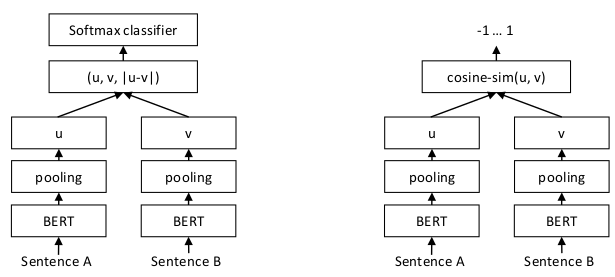
\includegraphics[width=0.8\linewidth]{sbert.png}
        \centering
        \caption[SBERT architectures]{SBERT architecture variants. 
        \textbf{Left}: classification objective function (softmax) and concatenation head (concatenating embeddings of both sentences and their element-wise difference resulting in $\mathbb{R}^{3n}$, where \emph{n} is the dimension of the sentence embedding).
        \textbf{Right}: regression objective function (MSE) and cosine similarity as head.~\parencite{Reimers_2019-SBERT}}
        \label{fig:sbert}
    \end{figure}
    
    Line of works motivated by the finding that sentence-level embeddings perform better when using transfer learning for downstream tasks than word-level embeddings~\parencite{cer2018universal} use this paradigm for training Sentence-BERT (SBERT)~\parencite{Reimers_2019-SBERT} model or TwinBERT~\parencite{lu2020twinbert}, which are dealing with the semantic search task. Their approach is to add a pooling layer to the BERT-like transformer, that generates fixed size embeddings. The pooling layer encodes sentence tokens from the input, over which it computes \emph{mean} or \emph{maximum} operation resulting in the sentence embedding. The network head and thus the final output together with the loss function depend on the available training data, examples of such architectures are shown in the Figure~\ref{fig:sbert}.
    
    Besides these examples, you can also use the triplet objective function, where the triples \emph{(query sentence, positive sentence, negative sentence)} are given. The network is tuned by the triplet loss (see equation~\ref{equ:triplet-loss}) such that the distance between the query and positive sentence is smaller than between the query and negative sentence. This approach provides a certain flexibility as the relevance between the query and a sentence does not necessarily be semantic, but for example thematic.~\parencite{ein-dor-etal-2018-learning}
    \begin{equation} 
        \label{equ:triplet-loss}
        \max(||s_q-s_p|| - ||s_q-s_n|| + \epsilon, 0)
    \end{equation}
    
    where:
    \begin{where}
        \item [|| \cdot ||] is Euclidean norm
        \item [\epsilon] is margin.
    \end{where}

    \begin{figure}[H]
        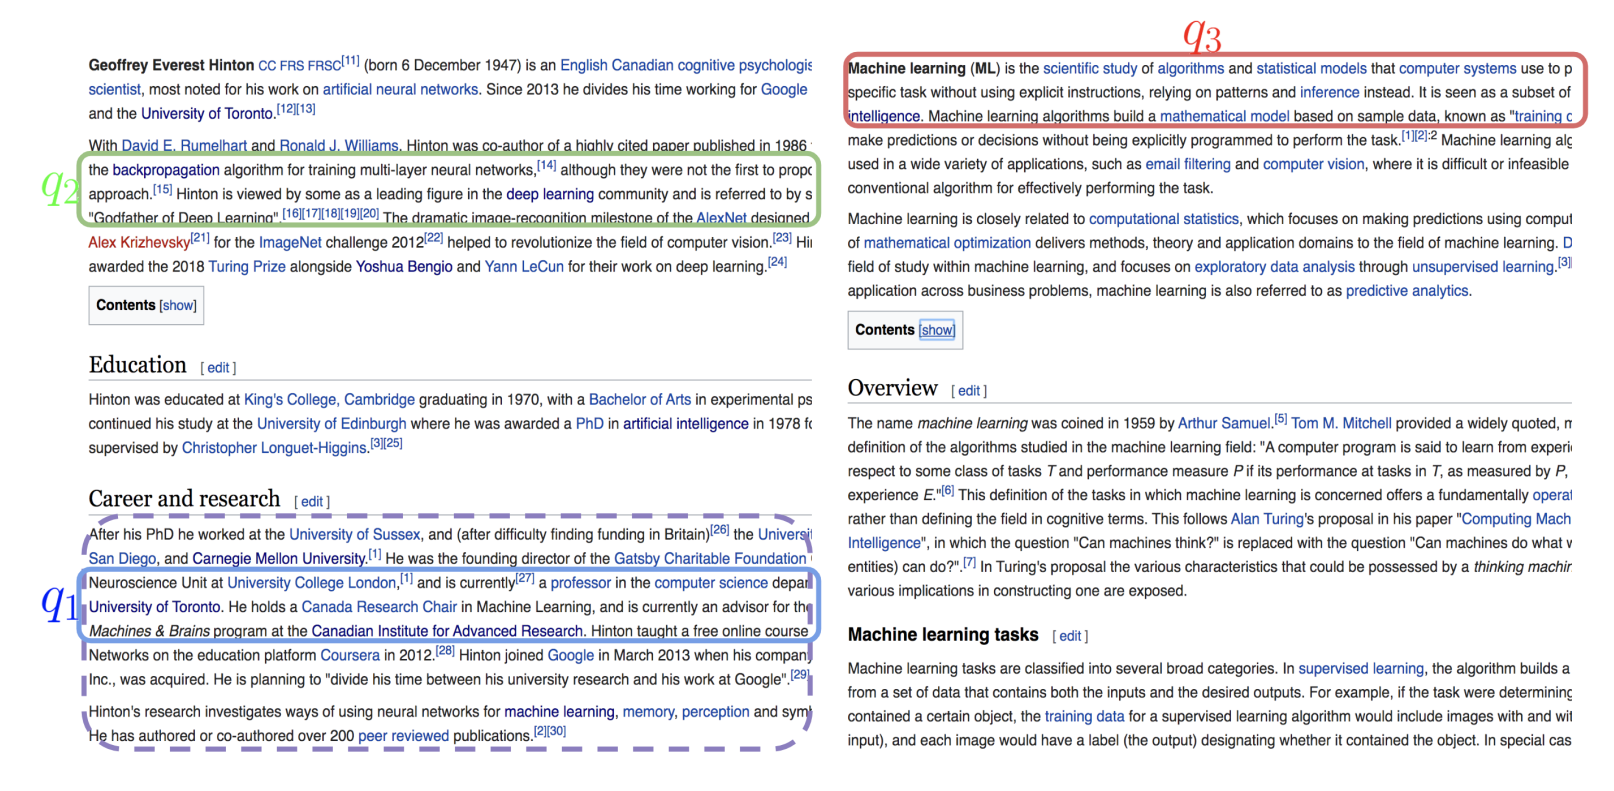
\includegraphics[width=1\linewidth]{2-tower-pretraining.png}
        \centering
        \caption[Pre-training tasks]{Example of the ICT, BFS, WLP pre-training tasks. Each randomly chosen sentence is denoted as a query and its corresponding paragraph (positive example) is denoted as \emph{d}. ICT is defined within a paragraph (\emph{q1}); BFS is defined globally within an article (\emph{q2}) and WLP is defined by hyperlinking a two Wikipedia articles through some entity (\emph{q3}).~\parencite{chang2020twotower}}
        \label{fig:two-tower-pretraining}
    \end{figure}

    LM's are usually pre-trained on MLM task or some similar task (see sections~\ref{section:multiling-models}~and~\ref{section:bertology}), which helps LM's to get general language comprehension, but this may not necessarily be sufficient for retrieval task. There are some works emphasizing the importance of further LM pre-training prior to application to downstream tasks to improve retrieval capabilities. In~\parencite{chang2020twotower}, they propose to further pre-train the LM on these paragraph-level retrieval relevant tasks:
    \begin{enumerate}
        \item \textbf{Inverse Cloze Task (ICT)} It was originally proposed in~\parencite{Lee_2019_ict}, where the task is supposed to capture the semantic context of a sentence. ICT randomly extracts a sentence from a passage \emph{p} and then tries to predict from what passage it comes (see Figure~\ref{fig:ict}).
        \item \textbf{Body First Selection (BFS)} It is supposed to capture semantic relationship outside of the local passage. BFS chooses a random sentence from the first summary paragraph of Wikipedia page (since it contains information central to the topic) and tries to classify a passage from the same document.
        \item \textbf{Wiki Link Prediction (WLP)} This task is proposed to capture inter-page semantic relation. It chooses a random sentence from the first summary paragraph of Wikipedia page and tries to classify a corresponding section from a linked page.
    \end{enumerate}

    \begin{figure}[H]
        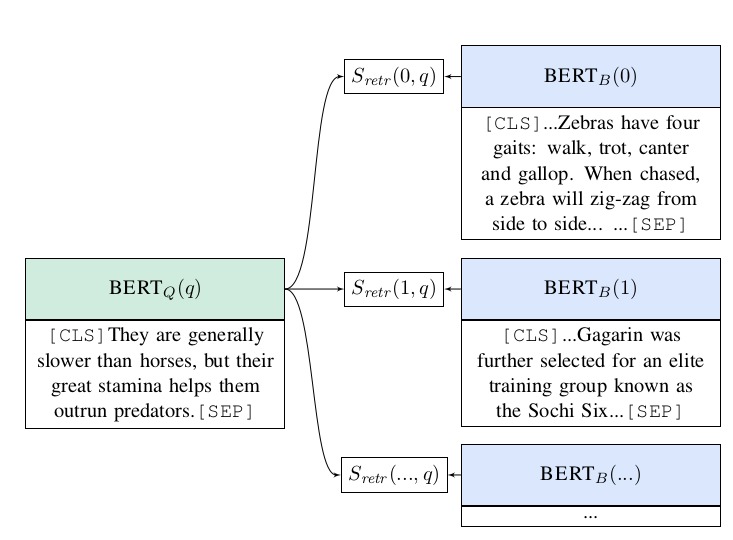
\includegraphics[width=0.8\linewidth]{ict.png}
        \centering
        \caption[Inverse Cloze Task]{ICT example used for retrieval pre-training. A random sentence (pseudo-query) and its context (pseudo evidence text) are derived from the text snippet: \textit{“...Zebras have four gaits: walk, trot, canter and gallop.} \textbf{They are generally slower than horses, but their great stamina helps them outrun predators.} \textit{When chased, a zebra will zig-zag from side to side...” The objective is to select the true context among candidates in the batch.}~\parencite{Lee_2019_ict}}
        \label{fig:ict}
    \end{figure}
    
    In this way, the further pre-trained transfomer model serves as method for converting queries and documents into common embeddings space. In the inference phase, relevant documents for a query are retrieved using nearest neighbors search (or its approximation for higher efficiency). In addition to the ability to capture deeper semantic relationships between query and documents, another advantage over traditional sparse-representation based approaches is the ability to optimize models for a given task.~\parencite{chang2020twotower} For completeness, there are also optimized and high-performing applications without involving any further pre-training step.~\parencite{ding2020rocketqa}


\subsection{Late Interaction Paradigm} \label{section:colbert}
    Late interaction paradigm (see Figure~\ref{fig:neural-approach-paradigms}~(d)) was presented in~\parencite{colbert_2020} and it tries to combine the benefits of the two previous paradigms. It enables fine-grained interaction of query and documents like the cross-attention setup, while the document representations can be precomputed offline. 
    
    It encodes each term of a query using BERT-based encoder into a bag of embeddings \emph{E\textsubscript{q}}. Similarly, it is done for each term of each document, which provides bag of fixed-sized embeddings \emph{E\textsubscript{d}}. Term refers to WordPiece token~\parencite{wordpiece-tokenizer}. Using those two bags of embeddings, the relevance score between \emph{q} and \emph{d} is computed as the sum of the maximum similarity between query term embeddings and document term embeddings. Particularly, for each term embedding from \emph{E\textsubscript{q}} is calculated similarity with all term embeddings from \emph{E\textsubscript{d}}, and only the highest (max) similarity is kept. By summing those maximum similarities for each query term, we get the desired relevance score between \emph{q} and \emph{d}.
    
    Instead of the maximum similarity operation, it is possible to use average similarity, or others. However, in the ColBERT paper~\parencite{colbert_2020} they strongly argue for the use of the maximum similarity operator due to its pruning-friendly nature, which is leveraged later in the retrieval process.
    %Further they experiment with cosine and L2 similarity metrics.
    %and average similarity instead of the maximum similarity operator.
    
    ColBERT model enables to re-rank already retrieved top-k documents or perform end-to-end top-k retrieval itself. Since the late interaction mechanism is specifically designed to enable end-to-end retrieval from a large collection with the goal to improve recall, it is the expected modus operandi. The retrieval utilizes a fast large-scale vector-similarity search from the FAISS~\parencite{Johnson_2019_faiss} library, which makes it possible to conduct the search between the query embedding and all document embeddings across the full collection efficiently. 
    
    When processing queries, the retrieval procedure consists of two parts to retrieve top-k most relevant documents from the collection. First, for each query term embedding from \emph{E\textsubscript{q}} is retrieved top-k' matches for that vector over all document embeddings. Each of those matched document term embeddings is then mapped to its document origin, which results in $N_{q} \times k'$ document IDs ($N_{q}$ = number of tokens in the query), while only K $\leq N_{q} \times k'$ of which are unique. These K documents probably contain one or more very similar embeddings to some query term embeddings. Efficiency of this step is ensured by the IVPF index from the FAISS library, which divides the indexing space into P partitions based on k-means clustering algorithm, so the document embeddings are mapped to their nearest clusters subsequently. This makes it possible to avoid a direct exhaustive search over all documents in the collection, by scoring only the documents from the nearest \emph{C} clusters.
    
    In the second step, only a relatively small number of documents K retrieved in the first step are exhaustively scored. Each document is represented by a matrix of embeddings (\#tokens $\times$ embedding dimension), which results in 3-dimensional tensor. The score of each document for a query \emph{q} is then calculated using the max-sim operator and summation over all query terms, a more detailed description can be found in the~\parencite{colbert_2020}. At the end, the documents are ranked according to their score. The obvious advantage over the cross-attention approach is that it is not necessary to calculate a relatively expensive attention for query \emph{q} and each document \emph{d} (N\textsubscript{q} + N\textsubscript{d} tokens), but only for the query \emph{q} (N\textsubscript{q} tokens).


\subsection{FAISS}
\label{section:faiss}
    Since both neural approaches (see~\ref{section:two-tower}~and~\ref{section:colbert}), we experimented with, use methods from the FAISS library~\parencite{Johnson_2019_faiss}, we will give a few words about it. FAISS is a library for efficient similarity search and clustering of dense vectors, developed by Facebook AI Research. It provides algorithms for search in sets of vectors of any size. It is highly optimized, which makes it fast and allows working with vectors that do not fit in RAM. It also contains supporting code for evaluation and parameter tuning. The library is written in C++ with optional GPU support provided via CUDA. It also provides complete wrappers for Python/numpy.
    
    FAISS contains several methods for similarity search and very efficient implementation of k-means clustering, PCA and product quantization. It works with instances represented as vectors, that can be compared with L2 (Euclidean) distance, dot product or cosine similarity\footnote{which is a dot product on normalized vectors}. The library offers several indexing structures ranging from direct ones that provide exact search to ones that involve some trade-off between search time, search quality, memory used per index, training time or need for external data for unsupervised training. 
    
    To give you an idea, some of the potential adjustments to the index are as follows. Faster search is possible by segmenting the database into Voronoi cells. At the search time, only the database vectors contained in the cell the query falls in and a few neighboring ones are compared against the query vector. Lowering memory footprint of an index is enabled by PCA or product quantization that will reduce the dimension to a configurable number. This will make possible to scale up even to very large datasets (billions of vectors).
    


\subsection{Long, Longer, Longest} %Handling Long Documents
\label{section:longformers}
    Along with the significant increase in the use of BERT-like transformers, its limits also became more apparent. One of them is a limited number of tokens at the input of the model as BERT operates with a maximum sequence length equal to 512 tokens. This is caused by an expensive self-attention mechanism. While powerful in performance, self-attention memory and computational requirements grow quadratically with sequence length, making it very costly or even infeasible to process long sequences using current hardware. Over the last two years, a number of works have appeared that address these limits and modify the attention mechanism. As this area of research opens up the possibility of working with long texts at the level of entire documents, we present a summary of it, as it can also have an effect on DR.
    
    The Longformer paper~\parencite{beltagy2020longformer} suggests to replace expensive self-attention with a combination of cheaper attention patterns (see Figure~\ref{fig:longformer-attention}). Specifically it uses local sliding window attention, dilated attention and global attention, which makes the Longformer to scale linearly with the input sequence length. They also propose a clever initialization scheme, that copies RoBERTa weights and absolute position embeddings into a Longformer version of RoBERTa with 8 times higher capacity supporting sequences of up to 4096 tokens in length. Using that simple yet effective idea makes the model pretraining to very quickly converge with a small number of gradient updates.
    \begin{figure}[H]
        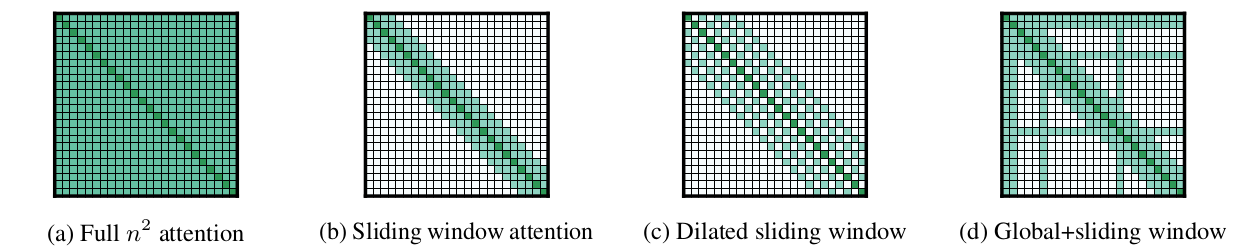
\includegraphics[width=1\linewidth]{longformer-attention.png}
        \centering
        \caption[Self-attention patterns]{Comparing the full self-attention pattern and the configuration of attention patterns used in Longformer.~\parencite{beltagy2020longformer}}
        \label{fig:longformer-attention}
    \end{figure}

    Another group of methods seeks to make the attention mechanism more efficient by approximating the full attention matrix with a lower rank matrix with size independent of the input length. The argument for this approach is based on the key observation that the self-attention is low rank.~\parencite{wang2020linformer} In other words, attention weights are dominated by a mere minority of key entries rather than being diffuse over the whole sequence. By performing spectral analysis, they showed that 90\% of the variation is explained by only the first 128 of 512 eigenvalues obtained by SVD.
    
    \begin{figure}[H]
        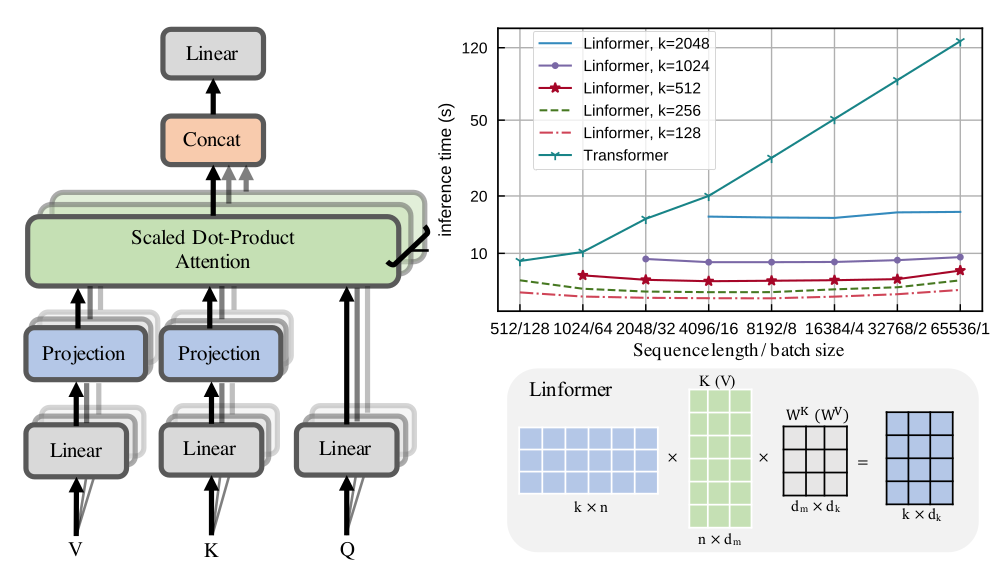
\includegraphics[width=0.8\linewidth]{linformer.png}
        \centering
        \caption[Linformer]{Left and bottom-right show architecture and example of the proposed multihead linear self-attention. Top right shows inference time vs. sequence length for various Linformer models.~\parencite{wang2020linformer}}
        \label{fig:linformer}
    \end{figure}
    
    Linformer model~\parencite{wang2020linformer} adds two linear projection matrices to the original self-attention (see the left part of the Figure~\ref{fig:linformer}). First, they project the original ($n \times d$)-dimensional key ($KW_{W}$) and value ($VW_{V}$) layers into ($k \times d$)-dimensional projected key and value layers. Then those two matrices are multiplied together to produce a ($n \times k$)-dimensional agreement matrix. Finally, multiplication of this agreement matrix (n, k) with the down-projected value matrix (k, d) will results in ($n \times d$)-dimensional just like in the original self-attention. By choosing a very small projected dimension k, such that $k \ll n$, makes the memory and space requirements significantly reduced. Computationally-wise, both computational and space complexity is linear with the respect to the sequence length \emph{n} (see the right side of the Figure~\ref{fig:linformer}).
    
    In addition to the above mentioned methods, there are a number of others using more or less different approaches, for example in the \emph{Routing transformer}~\parencite{Roy_2021} they decided to tackle this problem by k-means clustering. A nice overview capturing the development in this \enquote{making transformers more efficient} research direction and summarizing majority of the relevant work is provided in this survey~\parencite{long_survey_2020}. %Within our research group, this topic is further explored in the following work~\parencite{alex-mt}.

    % The limitation proceeds from the self-attention mechanism. Self-attention has both time and memory complexity $\mathcal{O}(n^2)$ and applying it over a long document can be prohibitive. This bottleneck can result in biased document retrieval models assessing shorter documents as more probable.~\parencite{hoffstater-long-1}
    